\chapter{Resultados}
\label{resultados}

\section{Modelos}
% \subsection{Random Forest}
% \textit{Random Forest} é um dos modelos de algoritmo mencionado no capítulo \ref{fund_teo}. Modelos \textit{Random Forests} são escolhidos para produzir boas previsões que são fáceis de entender. O fato de que pode lidar com grandes conjuntos de dados com eficiência e fornecer um alto nível de precisão geral é uma das razões pelas quais o escolhemos como um dos nossos modelos de aprendizado de máquina.

% \subsection{MLP}


% MLP é um modelo de perceptron mencionado no capítulo \ref{fund_teo}. Esta arquitetura é muito configurável, principalmente quando construída a partir de um framework como o Pytorch. No entanto, esta maleabilidade também proporciona muitos pontos de falha, como bugs ou dificuldades de implementação.

% Redes como o MLP tendem a lidar melhor com dados contínuos e a terem dificuldades em interpretar dados categóricos, o que traz outros desafios na adaptação do conjunto de dados para esta arquitetura.


% SUGESTÃO DO MLP 

% Redes Neurais MLP (Multi Layer Perceptron) são uma classe de redes neurais feedforward, também conhecidas como redes neurais densas ou simplesmente como redes neurais. Elas são compostas por várias camadas ocultas, cada uma composta por vários neurônios conectados por pesos sinápticos, que são ajustados durante o treinamento da rede.

% O funcionamento de uma rede neural MLP é simples: a entrada é passada através de cada camada da rede, sendo processada pelos neurônios de cada camada e transmitida para a próxima camada. A camada final é a camada de saída, que produz as previsões ou classificações para cada entrada.

% As redes MLP são usadas para uma ampla gama de tarefas, incluindo classificação de imagens, processamento de linguagem natural, análise de sentimentos e muito mais. Elas também são úteis como modelos de base para outras técnicas de aprendizado de máquina, como as redes neurais convolucionais e as redes neurais recorrentes.

% Em resumo, as redes neurais MLP são uma classe de redes neurais feedforward compostas por várias camadas ocultas, que são usadas para uma ampla gama de tarefas de aprendizado de máquina e são úteis como modelos de base para outras técnicas.

% sUGESTAO COM REFERENCIAS

% Redes Neurais MLP (Multi Layer Perceptron), também conhecidas como redes neurais densas ou simplesmente como redes neurais, são uma classe de redes neurais feedforward descritas detalhadamente em livros como "Redes Neurais - Uma Introdução" de Simon Haykin e "Deep Learning" de Ian Goodfellow, Yoshua Bengio e Aaron Courville. Estas redes são compostas por várias camadas ocultas, cada uma composta por vários neurônios conectados por pesos sinápticos, que são ajustados durante o treinamento da rede, descrito em detalhes em "Aprendizado de Máquina" de Tom Mitchell.

% O funcionamento de uma rede neural MLP é simples: a entrada é passada através de cada camada da rede, sendo processada pelos neurônios de cada camada e transmitida para a próxima camada, como descrito em "Redes Neurais Artificiais" de Albert Orriols-Puig e Joan Cabestany. A camada final é a camada de saída, que produz as previsões ou classificações para cada entrada.

% De acordo com "Aprendizado de Máquina" de Steven W. Rich et al., as redes MLP são usadas para uma ampla gama de tarefas, incluindo classificação de imagens, processamento de linguagem natural, análise de sentimentos e muito mais. Elas também são úteis como modelos de base para outras técnicas de aprendizado de máquina, como as redes neurais convolucionais e as redes neurais recorrentes, descrito em detalhes em "Deep Learning com Python" de François Chollet.

% Em resumo, as redes neurais MLP são uma classe de redes neurais feedforward compostas por várias camadas ocultas, descritas em livros como "Redes Neurais - Uma Introdução" e "Deep Learning", que são usadas para uma ampla gama de tarefas de aprendizado de máquina e são úteis como modelos de base para outras técnicas, descritas em detalhes em "Aprendizado de Máquina" e "Deep Learning com Python".


\subsection{LSTM}
\todo[inline]{isso não era pra estar mais na fund. teorica? ta mt introdutorio para esta sessão né}

Redes Neurais LSTM (Long Short-Term Memory) são uma classe de redes neurais recorrentes que foram projetadas para lidar com problemas de previsão de série temporal, como a previsão de bolsa de valores, clima, tráfego e outras sequências temporais. Uma das principais características das redes LSTM é sua capacidade de manter informações a longo prazo, enquanto descartando informações irrelevantes \cite{lstm-}. Isso é alcançado através da introdução de portas de controle de esquecimento e de atualização, que permitem ao modelo decidir quais informações manter e quais descartar.

O funcionamento das células LSTM consiste em três componentes: entrada, esquecimento e saída. A entrada é a informação que será processada pela célula, o esquecimento é o processo que controla quais informações serão retidas e quais serão descartadas e a saída é a informação transmitida para a próxima célula ou para a camada de saída da rede.

A vantagem desta arquitetura é que ela é capaz de lidar com dependências a longo prazo, ou seja, são capazes de lembrar informações relevantes ao longo de muitos passos no tempo, tornando-as muito úteis para a previsão de séries temporais.

De acordo com "Sequence Modeling with Deep Learning", as redes LSTM são usadas em uma ampla gama de tarefas, incluindo previsão de séries temporais, processamento de linguagem natural e geração de texto. Elas também têm aplicações em sistemas de reconhecimento de fala e em modelos de tradução automática, descritos em "Deep Learning for Speech and Language Processing" de Daniel Jurafsky e James Martin.

Em resumo, estas redes neurais são uma classe de redes neurais recorrentes projetadas para lidar com problemas de previsão de série temporal, baseadas em unidades LSTM que permitem que informações relevantes sejam retidas por períodos longos de tempo e informações irrelevantes sejam descartadas.

% SUGESTAO

% Redes Neurais LSTM (Long Short-Term Memory) são uma classe de redes neurais recorrentes descritas em detalhes em livros como "Deep Learning" de Ian Goodfellow, Yoshua Bengio e Aaron Courville e "Sequence Modeling with Deep Learning" de Jason Brownlee. Elas são usadas para processar sequências de dados, como séries temporais, texto e áudio, de forma mais eficaz do que as redes neurais MLP convencionais, descritas em "Redes Neurais - Uma Introdução" de Simon Haykin.

% Uma das principais características das redes LSTM é sua capacidade de manter informações a longo prazo, enquanto descartando informações irrelevantes, como descrito em "LSTM: A Search Space Odyssey" de Klaus Greff et al. Isso é alcançado através da introdução de portas de controle de esquecimento e de atualização, que permitem ao modelo decidir quais informações manter e quais descartar.

% De acordo com "Sequence Modeling with Deep Learning", as redes LSTM são usadas em uma ampla gama de tarefas, incluindo previsão de séries temporais, processamento de linguagem natural e geração de texto. Elas também têm aplicações em sistemas de reconhecimento de fala e em modelos de tradução automática, descritos em "Deep Learning for Speech and Language Processing" de Daniel Jurafsky e James Martin.

% Em resumo, as redes neurais LSTM são uma classe de redes neurais recorrentes descritas em detalhes em livros como "Deep Learning" e "Sequence Modeling with Deep Learning", usadas para processar sequências de dados e manterem informações a longo prazo, enquanto descartando informações irrelevantes. Elas são usadas em uma ampla gama de tarefas, incluindo previsão de séries temporais, processamento de linguagem natural e reconhecimento de fala, descritos em "Sequence Modeling with Deep Learning" e "Deep Learning for Speech and Language Processing".


\section{Metodologia}


%Por meio da biblioteca scikit-learn, é possível escrever um código simples que emprega o uso do modelo Random %Forest e com fácil customização. 

Podemos descrever o funcionamento do códigos de treinamento dos modelos por meio do seguinte fluxograma, na figura \ref{fig:rfflux}:

\begin{figure}[H]
	\centering
	\begin{minipage}{0.98\linewidth}
		\centering
		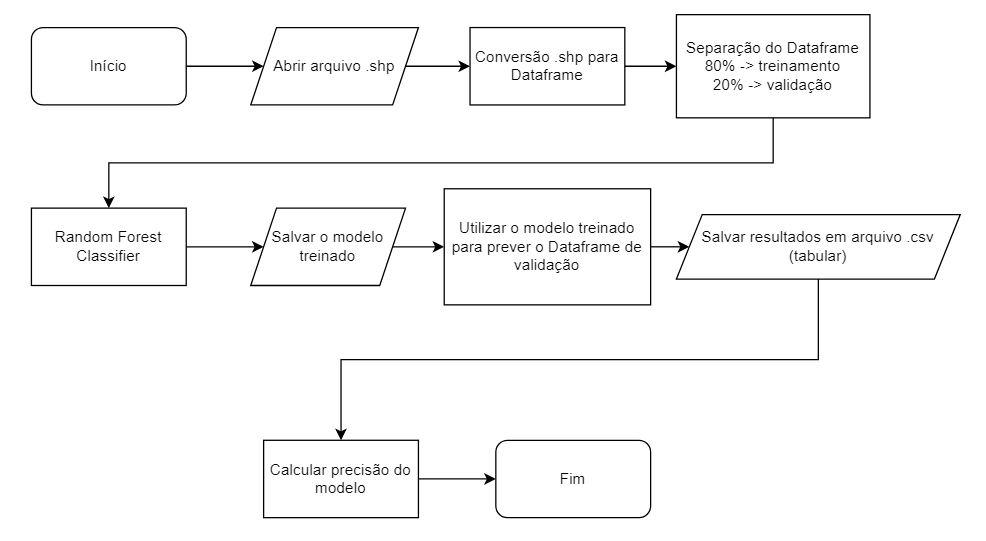
\includegraphics[width=\linewidth]{tg1/figuras/rfflux.png}
		\caption{Fluxograma do funcionamento do código do Random Forest} \label{fig:rfflux}
	\end{minipage}
\end{figure}
\todo{fluxograma do LSTM!!!}
Os parâmetros utilizados para a função do \textit{Random Forest Classifier} foram os valores padrões utilizados pelo scikit-learn \cite{sklearnrfc}, com o objetivo de obter-se um primeiro resultado para o nosso modelo. Enquanto os parâmetros do MLP foram sendo definidos até que a rede apresentasse \textit{overfitting}, demonstrando capacidade de generalização. Após isto, os seus hiper-parâmetros foram ajustados até fossem atingidos os melhores resultados encontrados.

\subsection{Lidando com Overfitting}
O problema de overfitting foi encontrado durante alguns testes como consequência do mal balanceamento do dataset. A classe 3, referente às queimadas de sub-bosque, representa 1.8\% do dataset, o que resulta em 0\% de acurácia para esta classe para um modelo treinando sem qualquer algoritmo de balanceamento.

É comum na literatura encontrar exemplos de "data augmentation" \cite{survey_data_augmentation}. Trata-se de algoritmos capaz de expandir um dataset sem comprometer de forma significativa seu valor como dado de treinamento. Neste trabalho, optou-se por empregar uma redução de dados como estratégia de balanceamento. Esta estratégia envolve eliminar de forma aleatória dados de rótulos diferentes de forma a se aumentar a representação do tipo de dados de menor presença no dataset. Este tipo de estratégia acabou resultando em overfitting, conforme a imagem a seguir.

\begin{figure}[ht]
    \centering
    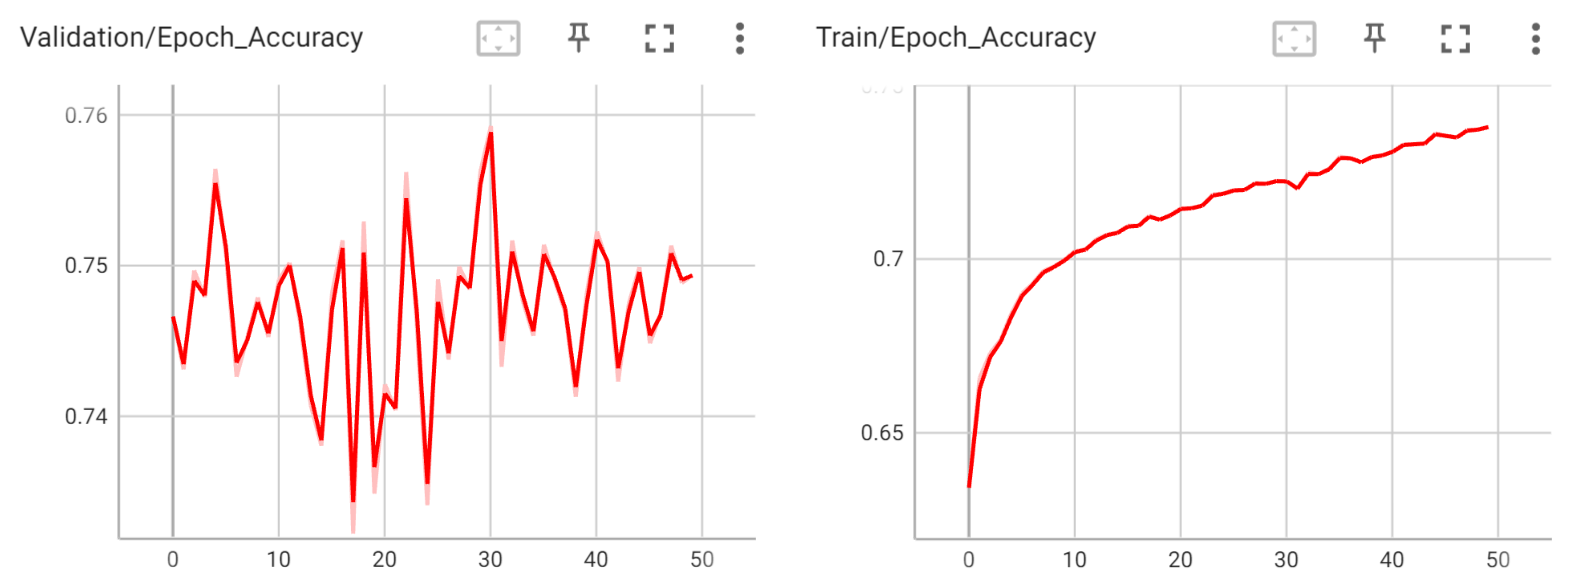
\includegraphics[scale=0.5]{tg1/figuras/overfit.png}
    \caption{Overfitting no treinamento}
    \label{fig:overfitting}
\end{figure}

Na figura \ref{fig:overfitting} pode-se ver que embora a acurácia de treinamento esteja aumentando, a acurácia de validação não está melhorando. Dessa forma, pode-se dizer que a rede está se tornando "viciada" nos dados de treinamento e aprendendo a interpretá-los bem mas não está aprendendo a interpretar dados estranhos.

Tendo em mãos estes resultados, optou-se por utilizar um leve balanceamento, aumentando a representatividade de 1.8\% para 5\%. Esta proporção foi obtida de forma empirica como um valor que representa uma melhora significativa na acurácia para a classe 3 porém sem reduzir demais a acurácia para as demais classes.


\subsection{Organização em Série Temporal}

Transformar os dados existentes em uma série temporal envolve a adição de uma nova dimensão, a temporal. Em termos práticos, isto é efetuado por meio de uma dimensão acrescentada aos tensores dos dados transformando eventos discretos em dados sequenciais. 

Os dados disponibilizados pelo CENSIPAM possuem identificadores rotulados como "id\_evento". Estes códigos agrupam diferentes detecções de incêndios como pertencentes a um mesmo foco de incêndio e é necessário para a transformação dos dados em uma série temporal. Em outras palavras, cada dados possui três dimensões: o ID representando o foco de incêndio, a quantidade de detecções relativas a este mesmo incêndio, e todos os dados de cada uma destas detecções.

No entanto, esta abordagem envolve o desafio de transformar estes dados em tensores. Todo o código utilizado é construído a partir do Pytorch \cite{NEURIPS2019_9015}, que utiliza tensores como tipo de dado. Tensores são matrizes multi-dimensionais, apenas uma forma de se organizar dados de forma lógica. Por exemplo, pode-se imaginar um tensor tridimensional como um cubo, tratando-se de um tensor cujo as três dimensões são iguais.

Em outras palavras, tensores são uma forma de se estruturar dados de forma regular, onde cada amostra de dados possui dimensões constantes e condizentes com as dimensões do tensor. No entanto, os dados em questão não são regulares pois são obtidos a partir de fenômenos aleatórios e caóticos, de queimadas sobre um território florestal de proporções continentais. Por isso é necessário o emprego de alguma técnica de tratamento de dados que possa regularizá-los, permitindo sua manipulação como tensores.

\subsubsection{Padding}

O desafio em questão é transformar dados de comprimento variado em dados padronizados com o mesmo comprimento, para que possam ser organizados como um tensor tridimensional. Dessarte, é necessário de se empregar um algoritmo capaz de preencher lacunas e eliminar excessos para garantir que todos os dados tenham as mesmas proporções.

"\textit{Padding}" não se trata de um algoritmo específico, mas de qualquer algoritmo capaz de preencher lacunas para garantir regularidade entre dados. Tratando-se de séries temporais, os algoritmos de \textit{Padding} mais comuns envolvem preencher com zeros, com médias ou repetindo valores. Neste trabalho, optou-se por preencher as lacunas repetindo-se a última detecção do evento e eliminando as primeiras em casos de eventos muito grandes. 

\begin{figure}[ht]
    \centering
    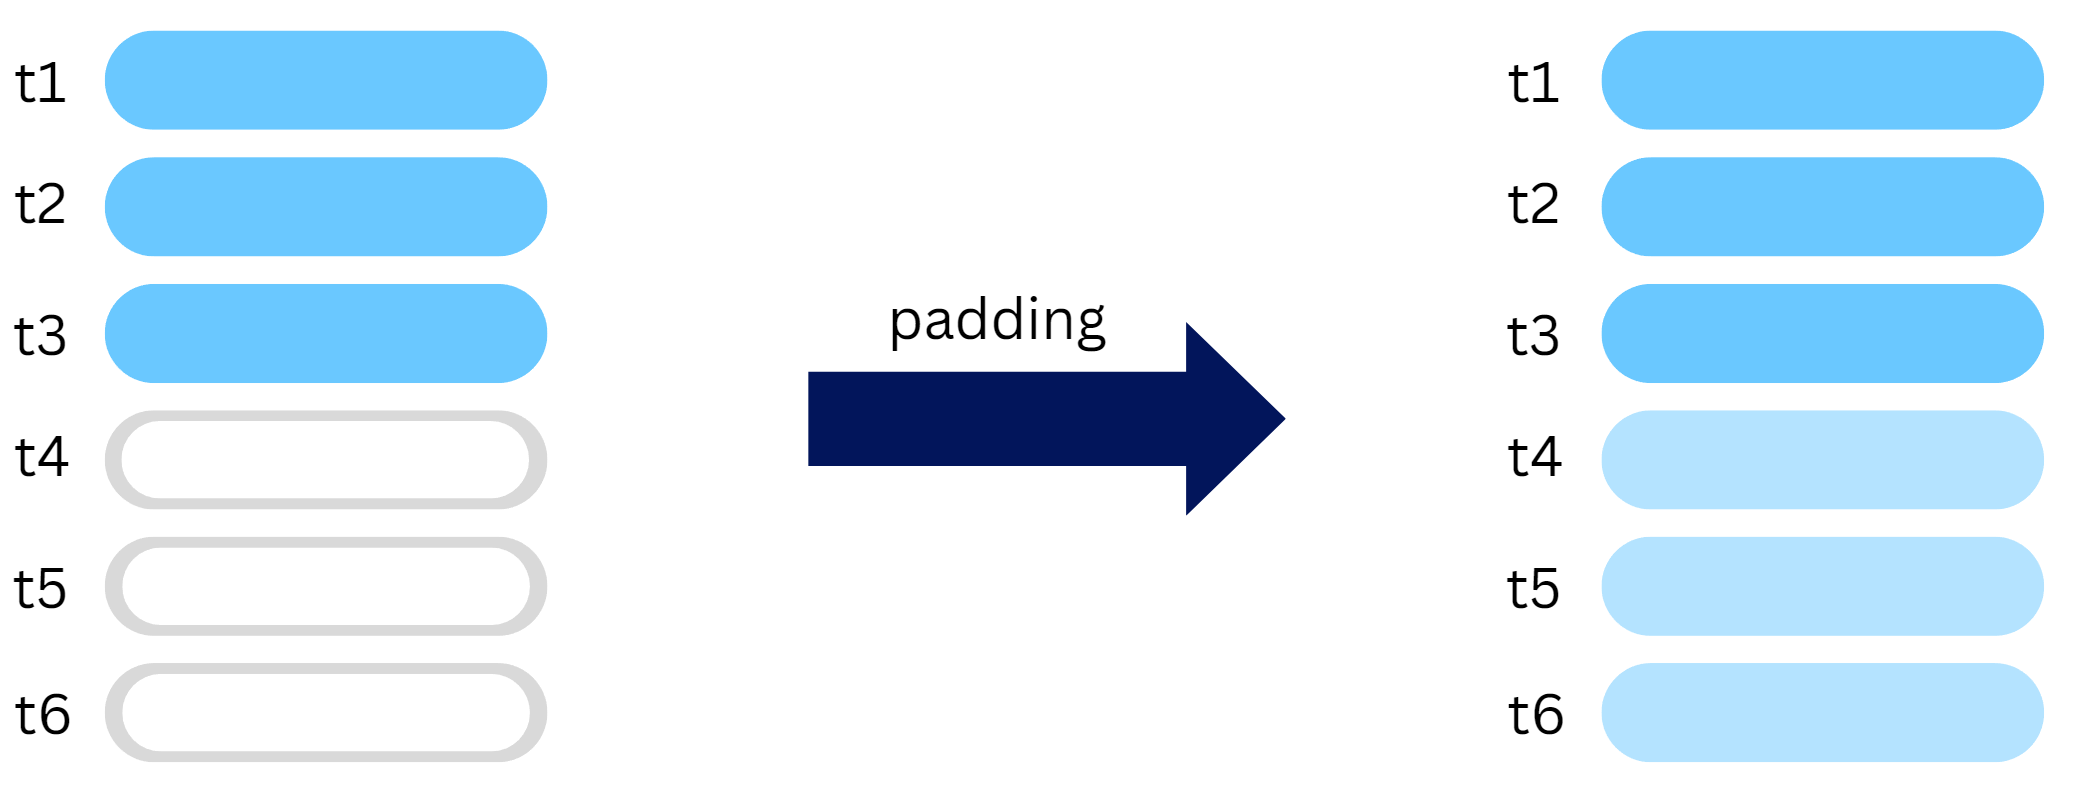
\includegraphics[scale=0.5]{tg1/figuras/padding.png}
    \caption{Representação de Padding}
    \label{fig:padding}
\end{figure}


O motivo para esta escolha é dado pela observação do comportamento da saída da rede ao longo de cada passagem pelos dados. Observou-se que a rede tende ajustar sua saída rapidamente, dentro de 5 iterações, e a manter esta saída até o final, revelando que converge em um valor rapidamente. Logo, foram evitados algoritmos que causem ruído no início da série temporal, período de maior convergência do algoritmo.

\subsection{Servidores do Censipam}
\subsection{Funcionamento em Produção}
\subsection{Treinamento x Produção}
\subsection{}



% \section{Evolução do modelo MLP}

% DROP OUT, NORM BATCH, LAYERS, BATCH SIZE, TREINAMENTO, MAQUINA UTILIZADA, ETC

% \section{Análise de Resultados}

% Na última etapa de calculo da precisão do modelo Random Forest, foi obtido os valores da tabela \ref{tab:rf} para quando classificamos o \textit{dataframe} de validação.

% \begin{table}[H]
% \caption{Precisão do modelo Random Forest}
% \label{tab:rf}
% \begin{tabular}{lllll}

%                  & Precision & Recall & F1-score & Quantidade \\
% 0                & 1.00      & 1.00   & 1.00     & 124125  \\
% 1                & 1.00      & 1.00   & 1.00     & 29652   \\
% 2                & 0.84      & 0.73   & 0.78     & 1866    \\
% 3                & 0.86      & 0.92   & 0.89     & 3615    \\
% Acurácia         &           &        & 0.99     & 159258  \\
% Média aritmética & 0.92      & 0.91   & 0.92     & 159258  \\
% Média ponderada  & 0.99      & 0.99   & 0.99     & 159258 
% \end{tabular}
% \end{table}


% A partir do resultado salvo em arquivo .csv, também é possível criarmos uma matriz de confusão para visualizarmos o comportamento da rede, conforme temos na figura \ref{fig:mcrf}. Quantos valores de cada tipo de fogo ela foi capaz de prever corretamente, e quantos ela errou, e para quais valores.

% \begin{figure}[htb]
% 	\centering
% 	\begin{minipage}{0.98\linewidth}
% 		\centering
% 		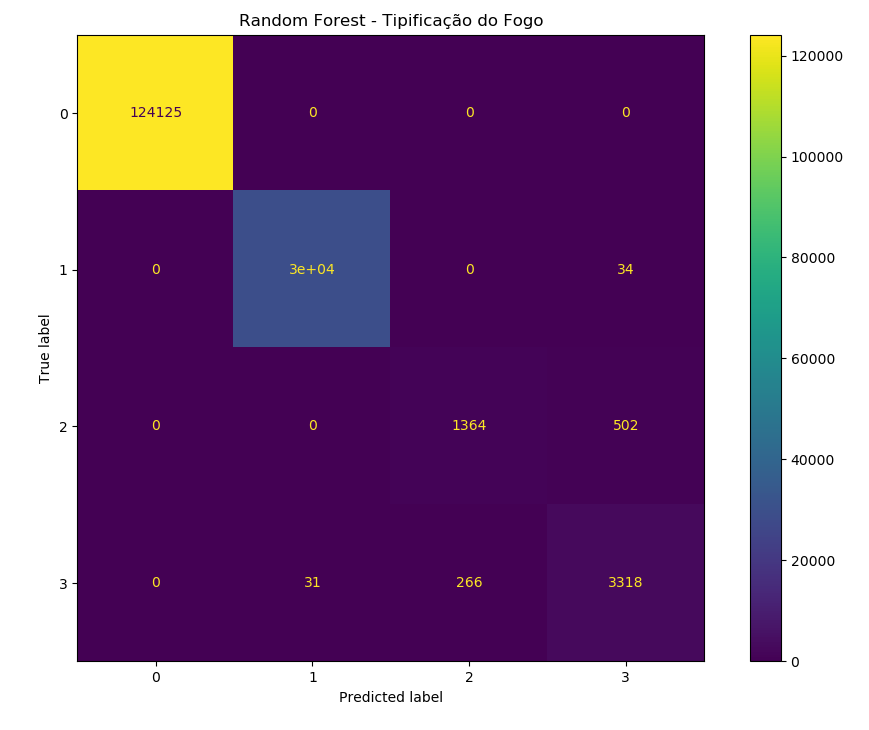
\includegraphics[width=\linewidth]{tg1/figuras/matrizconfusaorandomforest.png}
% 		\caption{Matriz de confusão para Random Forest} \label{fig:mcrf}
% 	\end{minipage}
% \end{figure}

% %\todo{COLOCAR METRICAS DO MLP}

% \begin{table}[H]
% \caption{Precisão do modelo MLP}
% \label{tab:rf}
% \begin{tabular}{lllll}

%                  & Precision & Recall & F1-score & Quantidade \\
% 0                & 1.00      & 1.00   & 1.00     & 124125  \\
% 1                & 0.98      & 1.00   & 0.99     & 29652   \\
% 2                & 0.69      & 0.66   & 0.68     & 1866    \\
% 3                & 0.79      & 0.84   & 0.81     & 3615    \\
% Acurácia         &           &        & ??     & 159258  \\
% Média aritmética & ??      & ??   & ??     & 159258  \\
% Média ponderada  & 0.99      & 0.99   & 0.99     & 159258 
% \end{tabular}
% \end{table}

